\documentclass{utfpr-pg}

\usepackage{cmap}
\usepackage[T1]{fontenc}
\usepackage{graphicx}
\usepackage{latexsym}
\usepackage{amssymb}
\usepackage{lipsum}

\graphicspath{{dummy/imagens/}}

\DeclareFloatingEnvironment[
fileext=lod,
listname=Lista de Definições,
name=Definição,
placement=tbhp,
]{definicao}

\departamento{Departamento Acadêmico de Informática}
\curso{Bacharelado em Ciência da Computação}
\autor{Nome Aluno}
\titulo{Titulo do trabalho de conclusão de curso}
\tipotrabalho{Trabalho de Conclusão de Curso}
\local{Ponta Grossa}
\data{2014}

\orientador{Nome Orientador}

\preambulo{\imprimirtipotrabalho\ apresentado como requisito parcial para obtenção do título de Bacharel em Ciência da Computação.}

% informações do PDF
\makeatletter
\hypersetup{
        % pagebackref=true,
        pdftitle={\@title},
        pdfauthor={\@author},
        pdfsubject={\imprimirpreambulo},
        pdfcreator={LaTeX with abnTeX2},
        colorlinks=false,
}
\makeatother

% Controle do espaçamento entre um parágrafo e outro:
\setlength{\parskip}{0.1cm}  % tente também \onelineskip

\makeindex
\begin{document}
% Retira espaço extra obsoleto entre as frases.
\frenchspacing

\imprimircapa
\imprimirfolhaderosto

 \begin{resumo}
   \refthis{dummy}
   \lipsum[23]
   \vspace{\onelineskip}
   \noindent
   \textbf{Palavras-chaves}: palavras. chaves. quico.
 \end{resumo}

 \begin{resumo}[Abstract]
   \begin{otherlanguage*}{english}
   \refthis[en]{dummy}
     This is the english lipsum. \lipsum[2]
     \vspace{\onelineskip}
     \noindent
     \textbf{Key-words}: latex. abntex.
   \end{otherlanguage*}
 \end{resumo}


% \pdfbookmark[0]{\listfigurename}{lof}
% \listoffigures*
% \cleardoublepage

% \pdfbookmark[0]{\listtablename}{lot}
% \listoftables*
% \cleardoublepage

% \begin{siglas}
% \item[Fig.] Area of the $i^{th}$ component
% \item[456] Isto é um número
% \end{siglas}

% \begin{simbolos}
% \item[$ \Gamma $] Letra grega Gama
% \end{simbolos}

\pdfbookmark[0]{\contentsname}{toc}
\tableofcontents*
\cleardoublepage

\textual
\pagestyle{simple}

\chapter{Introdução}
\lipsum[1]
\cite{kwiatkowska_probabilistic_2002}.

\section{Objetivos}
Os objetivos deste trabalho são:
\begin{itemize}
\item \lipsum[2]
\item \lipsum[3]
\end{itemize}

\section{Justificativa}
\lipsum[4-7] \cite{gummalla}.

\chapter{Fundamentação teórica}
\lipsum[2-4] \cite{wing98}.

\section{Especificação formal}
\lipsum[7-9]
\subsection{Domínio sintático}
\lipsum[10-11]
\subsection{Domínio semântico}
\lipsum[12-15]
\subsubsection{Verificação formal}
\lipsum[16-17]
\subsubsubsection{O problema da explosão de estados}
\lipsum[20-27]

\chapter{Model Checking}

A maioria dos problemas encontrados são problemas clássicos de concorrência, como processos rodando de maneira alternada e acessando variáveis compartilhadas \cite{Katoen08}. Um exemplo básico desta situação é o exposto na figura \ref{fig:interleaving}. Considere um sistema com os três processos descritos na figura rodando em paralelo. O objetivo do sistema, conforme descrito informalmente, seria manter o valor da variável $\mathit{x}$ entre 0 e 200, inclusive.
\begin{figure}[h]
  \centering
  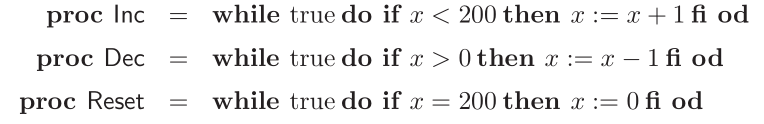
\includegraphics[scale=.5]{interleaving.png}
  \caption{\textbf{Três processos rodando de maneira concorrente.}}
  \fonte{\textbf{\citeonline[pg. 10]{Katoen08}}}
  \label{fig:interleaving}
\end{figure}

A princípio, este programa faz o que foi especificado, o processo \textsf{Inc} mantém a variável aumentando em direção a 200; \textsf{Dec} a mantém diminuindo em direção a 0; e \textsf{Reset} retorna $\mathit{x}$ a 0 quando o valor 200 for atingido. O problema com o código acima, que provavelmente passou despercebido ao leitor, bem como ao programador que o escreveu é o fato de que como os processos rodam em paralelo, de maneira concorrente com relação à variável $\mathit{x}$, pode ocorrer a seguinte situação: suponha que o valor de $\mathit{x}$ em um dado momento é 200. O processo \textsf{Dec} efetua a comparação ($\mathit{x} > 0$) e o teste é avaliado para verdadeiro. Neste momento, o processo \textsf{Reset} também faz a sua comparação ($\mathit{x} = 200$) e como o teste também avalia para verdadeiro, prossegue com a execução do bloco e reinicia a variável $\mathit{x}$ para 0. \textsf{Dec}, então, continua sua execução, e como o seu teste já havia passado, executa o seu bloco de código e decrementa $\mathit{x}$, colocando o sistema em um estado inesperado ($\mathit{x} = -1$) e potencialmente inconsistente e incorreto.

\section{Propriedades}
\lipsum[55]

\subsection{Vantagens e desvantagens}
A seguir, estão listadas algumas das vantagens e desvantagens do com relação às outras técnicas de verificação como a prova de teoremas, simulação e teste.

Segundo \citeonline{Clarke_2008}:

\noindent
\begin{minipage}[t]{0.49\columnwidth}%
\noindent \textbf{Vantagens:}
\begin{itemize}
\item Não é necessário fazer provas.
\item É uma técnica rápida.
\item Produz contra-exemplos.
\item Permite especificações parciais.
\item A lógica temporal tem boa expressividade dos conceitos de programas concorrentes.
\end{itemize}
\end{minipage}%
\begin{minipage}[t]{0.49\columnwidth}%
\textbf{Desvantagens:}
\begin{itemize}
\item Provas podem ajudar a entender melhor um programa.
\item Especificações em lógica temporal podem ficar muito complexas.
\item É difícil escrever especificações.
\item O problema da explosão de estados.
\end{itemize}
\end{minipage}

\section{Autômato temporal}
Para fins de completude, a definição formal de um autômato temporal é apresentada na definição \ref{ta} \cite{secret}.

\begin{definicao}
  \captionsetup{justification=raggedright,
singlelinecheck=false
}
  \caption{Autômato temporal}
  \label{ta}
  Seja $\mathit{C}$ um conjunto de relógios e $\mathit{x},\mathit{y} \in C$; $\mathit{c}\in\mathbb{N}$; $op\_rel \in \{\leq,\geq,=,<,>\}$; define-se $B(C)$ como um conjunto de \textit{guards}, onde \textit{guard} é uma conjunção da forma $\mathit{x}\ op\_rel\ \mathit{c}$ ou $\mathit{x}-\mathit{y}\ op\_rel\ \mathit{c}$.    
\end{definicao}

% Finaliza a parte no bookmark do PDF, para que se inicie o bookmark na raiz
\bookmarksetup{startatroot}%

% \chapter*[Conclusão]{Conclusão}
% \addcontentsline{toc}{chapter}{Conclusão}

\postextual
\bibliography{dummy}

% \begin{apendicesenv}
%   %   Imprime uma página indicando o início dos apêndices
%   \partapendices
%   \chapter{Quisque libero justo}
%   \chapter{Nullam elementum urna vel imperdiet sodales elit ipsum pharetra ligula
%   ac pretium ante justo a nulla curabitur tristique arcu eu metus}
% \end{apendicesenv}

% \begin{anexosenv}
%   %   Imprime uma página indicando o início dos anexos
%   \partanexos
%   \chapter{Morbi ultrices rutrum lorem.}
%   \chapter{Cras non urna sed feugiat cum sociis natoque penatibus et magnis dis
%   parturient montes nascetur ridiculus mus}
%   \chapter{Fusce facilisis lacinia dui}
% \end{anexosenv}
\end{document}
